\vspace{1.5 cm}}
\section{Análise de Desempenho Analítica\label{section:context}}
% What is the problem being worked on?
% What was the state-of-the-art before the paper was written?
% What impact did the paper have (if known)? 

\justifying
\noindent
\subsubsection{Questão 1}
\vspace{0.5cm}
\begin{center}
    \begin{tabular}{r|lr}
        Número de Instruções & Valores \\ % Note a separação de col. e a quebra de linhas
        \hline                               % para uma linha horizontal
        Inteiro        & ${4x10^{11}}$ \\
        Float  & ${1,6x10^{12}}$ \\
    \end{tabular}
    \strut
    \begin{tabular}{r|lr}
        Número de Acessos a Memória  & Valores \\ % Note a separação de col. e a quebra de linhas
        \hline                               % para uma linha horizontal
        L1 & ${72x10^{5}}$ \\
        L2 & ${15x10^{5}}$\\
        Memória Primária & ${13x10^{5}}$
    \end{tabular}
\end{center}
\vspace{0.5cm}

Obs: A fim de reduzir o número de páginas, optamos por não deixar os esboços dos cálculos.  

\vspace{0.5cm}
\begin{center}
    \vspace{0.2cm}
    \centering
    \begin{small}
         \textbf{Tabela sobre Tempo gasto para executar o programa BABE} \label{Tabela1}
        \hline
         \vspace{0.5cm}
            \begin{tabular}{|c|c|}
            \hline
            Computadores            & Valores\\
            \hline
            Computador A                 & 140.8s \\
            Computador B                 & 128.8s \\
            Computador Referência        & 29.29s \\
            \hline
        \end{tabular}
    \end{small}
    
\end{center}
\vspace{0.5cm}

\subsubsection{Questão 2}
\vspace{0.5cm}
\begin{center}
    \vspace{0.2cm}
    \centering
    \begin{small}
         \textbf{Speedup do Computador de Refêrencia em relação aos outros} \label{Tabela1}
        \hline
         \vspace{0.5cm}
            \begin{tabular}{|c|c|}
            \hline
            Computadores            & Valores\\
            \hline
            Computador A/Ref             & 4.8x \\
            Computador B/Ref             & 4.4x \\
            \hline
        \end{tabular}
    \end{small}
    \centerline{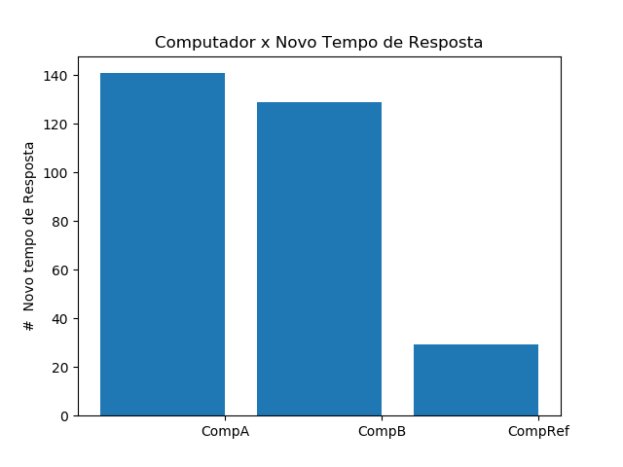
\includegraphics[width=120mm]{images/speedup.png}}
    \centerline{Figura 4: Gráfico referente ao speedup}
\end{center}
\vspace{0.5cm}

\subsubsection{Questão 3}
O computador BEST escolhido foi o computador de referência, haja visto que foi o computador que executou o programa em menor tempo.
\end{center}
\vspace{0.5cm}
\subsubsection{Questão 4,5 e 6}
\vspace{0.5cm}
\begin{center}
    Usamos uma mesma tabela para as questões 4, 5 e 6, visto que elas usam os mesmos cálculos para o tempo final modificando apenas os valores da memória.
    
    \vspace{0.5cm}
    \centering
    \begin{small}
         \textbf{Tempo de resposta sem a L2, apenas com a memória principal e apenas com a cache L2} \label{Tabela1}
        \hline
         \vspace{0.5cm}
            \begin{tabular}{|c|l|c|}
            \hline
            Computadores            & Tempo & Desempenho\\
            \hline
            Computador Ref4             & 29.353s & 0.063s pior \\
            Computador Ref5             & 29,628s & 0.338s pior\\
            Computador Ref6             & 29,261s & 0.029s melhor\\
            \hline
        \end{tabular}
    \end{small}
    
\end{center}
\vspace{0.5cm}

\subsubsection{Questão 7}
O Computador de referência possui 1 MB de cache L2 e 16 GB de RAM, fazendo a conversão temos 16000 MB de RAM. Percebe-se que seriam necessários 15999 MB de memória para que a cache L2 tenha a mesma quantidade de memoria que a RAM, assim para saber o preço basta fazer o cálculo: 15999 * 50 = 799950 reais. Ou seja, o ganho de desempenho não vale o custo adicional.

\subsubsection{Questão 8}
\vspace{0.5cm}
\begin{center}
    \vspace{0.2cm}
    \centering
    \begin{small}
         \textbf{Tempo de resposta para diferentes quantidades de ULAs e UPFs} \label{Tabela1}
        \hline
         \vspace{0.5cm}
            \begin{tabular}{|c|l|c|}
            \hline
            Qtd de processadores            & ULAs & UPFs\\
            \hline
            2             & 1.96s  & 12.65s\\
            4             & 0.98s  & 6.325s\\
            8             & 0.49s    & 3.1625s\\
            16            & 0.245s      & 1.58125s\\  
            \hline
        \end{tabular}
    \end{small}
\end{center}
\centerline{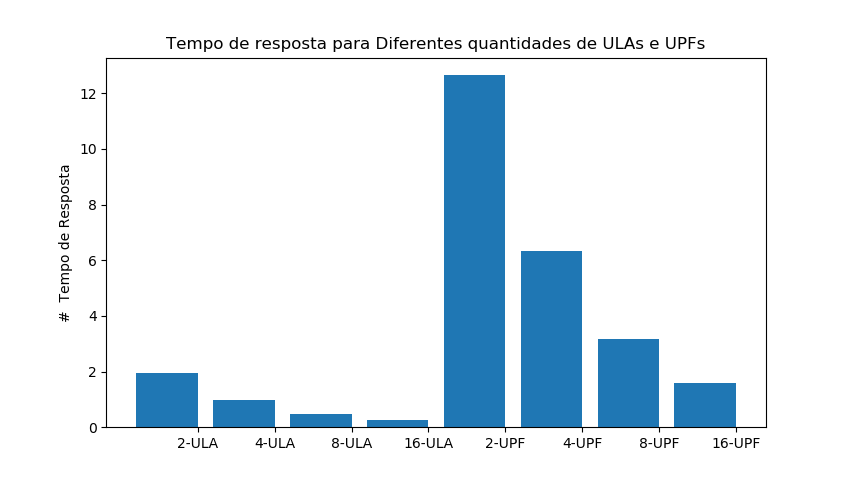
\includegraphics[width=180mm]{images/performance_gain.png}}
\centerline{Figura 5: Gráfico referente aos valores de ULA e UPF}
\vspace{0.5cm}

\subsubsection{Questão 9}
\vspace{0.5cm}
\begin{center}
    \vspace{0.2cm}
    \centering
    \begin{small}
         \textbf{Ganho no tempo de resposta em cada computador} \label{Tabela1}
        \hline
         \vspace{0.5cm}
            \begin{tabular}{|c|c|}
            \hline
            Computadores            & Ganho\\
            \hline
            CompA             & 63.63s\\
            CompB             & 58.4s\\
            CompRef             & 12.652s\\
            \hline
        \end{tabular}
    \end{small}
\end{center}
\subsection{Questão 10}
\centerline{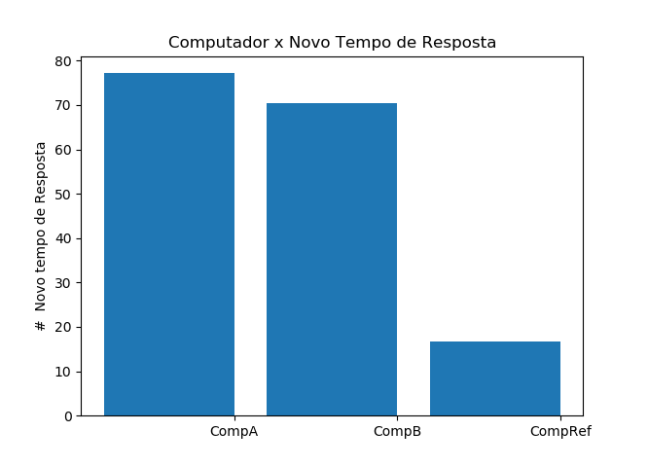
\includegraphics[width=120mm]{images/new_gain.png}}
\centerline{Figura 6: Gráfico referente aos novos valores do tempo de resposta}
\vspace{0.5cm}
\subsection{Questão 11}
Mesmo após todas as modificações o computador de referência manteve-se com desempenho superior aos demais.
\section{Conclusão}
Considerando as medidas e análises realizadas neste trabalho, concluimos que o computador de referência se destacou entre os demais em todos os aspectos. Programas com ênfase em análise de dados, jogos(como jogos de mundo aberto por exemplo), processamento gráfico, edição de vídeos e visão computacional são exemplos de usos em que o computador de referência teria um desempenho melhor do que os outros.
\par
Conforme vimos nos benchmarks feitos podemos ressaltar algumas vantagens como o Geekbench(\cite{CPUcompA} e \cite{CPUcompB}) em que o benchmark é feito de forma rápida porém com resultados superficiais, já o Sisoftware Sandra possui resultados melhores e mais detalhados porém com uma interpretação mais complexa, com uma maior exigência computacional e longo tempo de duração.
\par
Através dos cálculos feitos nesse trabalho pode-se ressaltar algumas métricas importantes para comparar a análise de desempenho de cada computador, por exemplo: a memória primária, memória cache, a frequência de clock, a latência e o número de MIPS e MFLOPS. Vale dizer também que essas métricas só serão úteis se forem analisadas em conjunto, por exemplo, não é só porque um computador possui um valor de MIPS maior do que o outro que ele será melhor.
\par
Portanto, pode-se concluir que o resultado que mais surprendeu o grupo foi o tempo de execução do programa BABE no computador de referência, haja visto que este obteve um tempo bem melhor em relação as outras máquinas.
\vspace{8.0cm}
%-------------------------------------------------------------------

\end{text}